\documentclass[11pt, a4paper,titlepage]{article}
\usepackage[utf8]{inputenc}
\usepackage{lipsum}
\usepackage{latexsym}
\usepackage{hyperref}
\usepackage[left=2.35cm, right=3.35cm, top=3.35cm, bottom=3.35cm]{geometry}
\usepackage[english]{babel}
\usepackage{graphicx}
\usepackage{titlesec}
\usepackage{tocbibind}

\begin{document}

\begin{titlepage}
  \begin{center}
    
    
\includegraphics[scale=1.5]{Figures/kuleuven_logo.pdf}~\\[4.5cm]
    
    \textsc{\Large Integrated Bioinformatics Project}\\[0.5cm]
    
    % Title
    \rule{\linewidth}{0.3mm}\\[0.4cm]
    {\huge \bfseries Assignment} \\[0.4cm]
    {\large Fall 2015} \\[0.4cm]
    \rule{\linewidth}{0.3mm}\\[1.5cm]
    
    % Author and supervisor
    \begin{minipage}{0.4\textwidth}
      \begin{flushleft} \large
        \emph{Author:}\\
        Hamed \textsc{Borhani}\\
		MohamedHakim \textsc{Elakhrass}\\
		Yi Ming \textsc{Gan}\\
		Cedric \textsc{Lood}
      \end{flushleft}
    \end{minipage}
    \begin{minipage}{0.4\textwidth}
      \begin{flushright} \large
        \emph{Supervisors:} \\
        Prof. Jan \textsc{Aerts}\\
        Prof. Rob \textsc{Lavigne}
      \end{flushright}
    \end{minipage}
    
    \vfill
    
    
\includegraphics[scale=0.15]{Figures/KUL.jpg}~\\[0.5cm]

    % Bottom of the page
    {\large \today}
    
  \end{center}
\end{titlepage}


\section{Introduction}

Clustered, Regularly Interspaced, Short Palindromic Repeats (CRISPR)
and CRISPR-associated proteins (Cas proteins) form a complex
bacterial/archaeal immune response system that mitigates foreign DNA
activity. The identification of these systems first occured in 1987 in
\emph{Escherichia coli} \cite{nakata1989unusual}, followed by other
species of bacteria and archae \cite{mojica1995long}, but their
function was not elucidated until 2007 \cite{Barrangou23032007}. This
immune-like system works by capturing short signatures of invading DNA
and inserting them into the genomic material in regions known as
CRISPR arrays.

These arrays consist of the captured elements, known as spacers, which
are separated by similarly sized, conserved DNA sequences known as
repeats.  The arrays are transcribed and processed into CRISPR RNA
(crRNA). crRNA, together with Cas proteins, form an active complex
that patrols the cell. If an invader DNA element with a similar
signature is encountered by the complex, it will be degraded and its
activity will be prevented \cite{Horvath08012010}.

CRISPR-Cas systems can be categorized into multiple types. Each type
having a different set of features that makes it somewhat unique
\cite{makarova2011evolution}.

Previously \cite{Omicians2015}, our team used computational CRISPR
detection software like CRT \cite{bland2007crispr} to detect spacers
from all ``reference'' bacterial and archael genomes on NCBI (about
5000 genomes in total in May 2015) . A subsequent step had been to
blast those detected elements against the NCBI nucleotide
database. This revealed the origin of about 7\% of spacers, outlining
the problem of the so-called \emph{biological dark matter}. The
identified spacers were also searched against the genomes of the
bacteria they originated from. Spacers showing up outside of the
CRISPR region were classified as \emph{hits}. Hits putatively showed
that there was a possibility for given phages to integrate into
bacterial genome despite the presence of spacers against them.

The main objective of this project was to make a large database of
CRISPR elements from all the bacterial/archaeal genomes available in
the NCBI genome database. Hence, removing the limitations we had
before when we focused only on ``reference genomes''. The number of
genomes considered is thus substantially higher, about 54000 at the
time of this project (December 2015). A database of these elements was
made accessible via a web application. The associated website exposes
the CRISPR details of the strains, along with a number of services,
such as blasting against spacer elements, CRISPR array detection, and
elements of data visualization.

\section{Methods and results}

\subsection{Classification of CRISPR-Cas systems}
We attempted to classify CRISPR-Cas systems based on methods proposed
by Makarova \emph{et al.}. The data set from their studies (supplementary document
7) was first processed into a clean subset (without “partial” subtypes
and ambiguous classification) to search for possible classifiers. Loci
were classified as “partial” if they contained neither the full
complement of effector module genes nor \emph{cas9} or \emph{cpf1}. The
classification criteria was polythetic classification as mentioned in
their studies \cite{makarova2015updated}.

Two approaches were attempted to tackle the problem, random forest and
Naive Bayes. Random forest showed unpromising results as the total
factor level exceeded computational limit. On the other hand, Naive
Bayes model performed well with the clean dataset with overall
accuracy of 0.98, high sensitivity and specificity to all subtypes
except lower sensitivity to CAS-I-A (0.85) and CAS-III-C (0.93) in the
validation set.

The task proved to be non-trivial and was eventually discontinued due
to time constraint. Challenges encountered in the process include
ambiguous classification, need for a pipeline to detect and annotate
cas genes, and genomes bias etc.

\subsection{Data Processing Pipeline}

The first step of the data processing pipeline was to gather all
possible bacterial and archaeal genomes available from the NCBI genome
database. This task was accomplished using a custom python script
which fetched from the RefSeq ftp site \cite{pruitt2007ncbi} the 54000
prokaryote genomes available (all assembly levels). In practice that
meant downloading the genome files (*.fna). Alongside each genome
file, the corresponding annotation files (*.gff) were also
downloaded. Finally the corresponding metadata available on NCBI for
each genome was captured into JSON files. All the files, representing
about 300 Gb worth of data were stored in a ``one genome, one folder''
fashion on our server.

The second step was to detect all CRISPR arrays (i.e spacers and
repeats) in each genome. For this, the CRT software
\cite{bland2007crispr} was used. In order to treat the the multi-FASTA
files correctly (e.g for genomes containing plasmid sequences, or
multiple contigs) the CRT software was wrapped in a python script and
then applied to the fetched genomes to create the CRT report files
containing detected CRISPR array(s) in each strain. Next, a custom
parser was implemented to extract the spacers and repeats from each
CRT report and structure them into a JSON file.

These CRISPR elements and the metadata fetched previously were used to
populate the relational MySQL database. All spacers available were
extracted from the MySQL database and consolidated into a multi-FASTA
file and a blastable database was made using the \emph{formatdb} tool
from the NCBI BLAST.

\begin{figure}
  \centering
  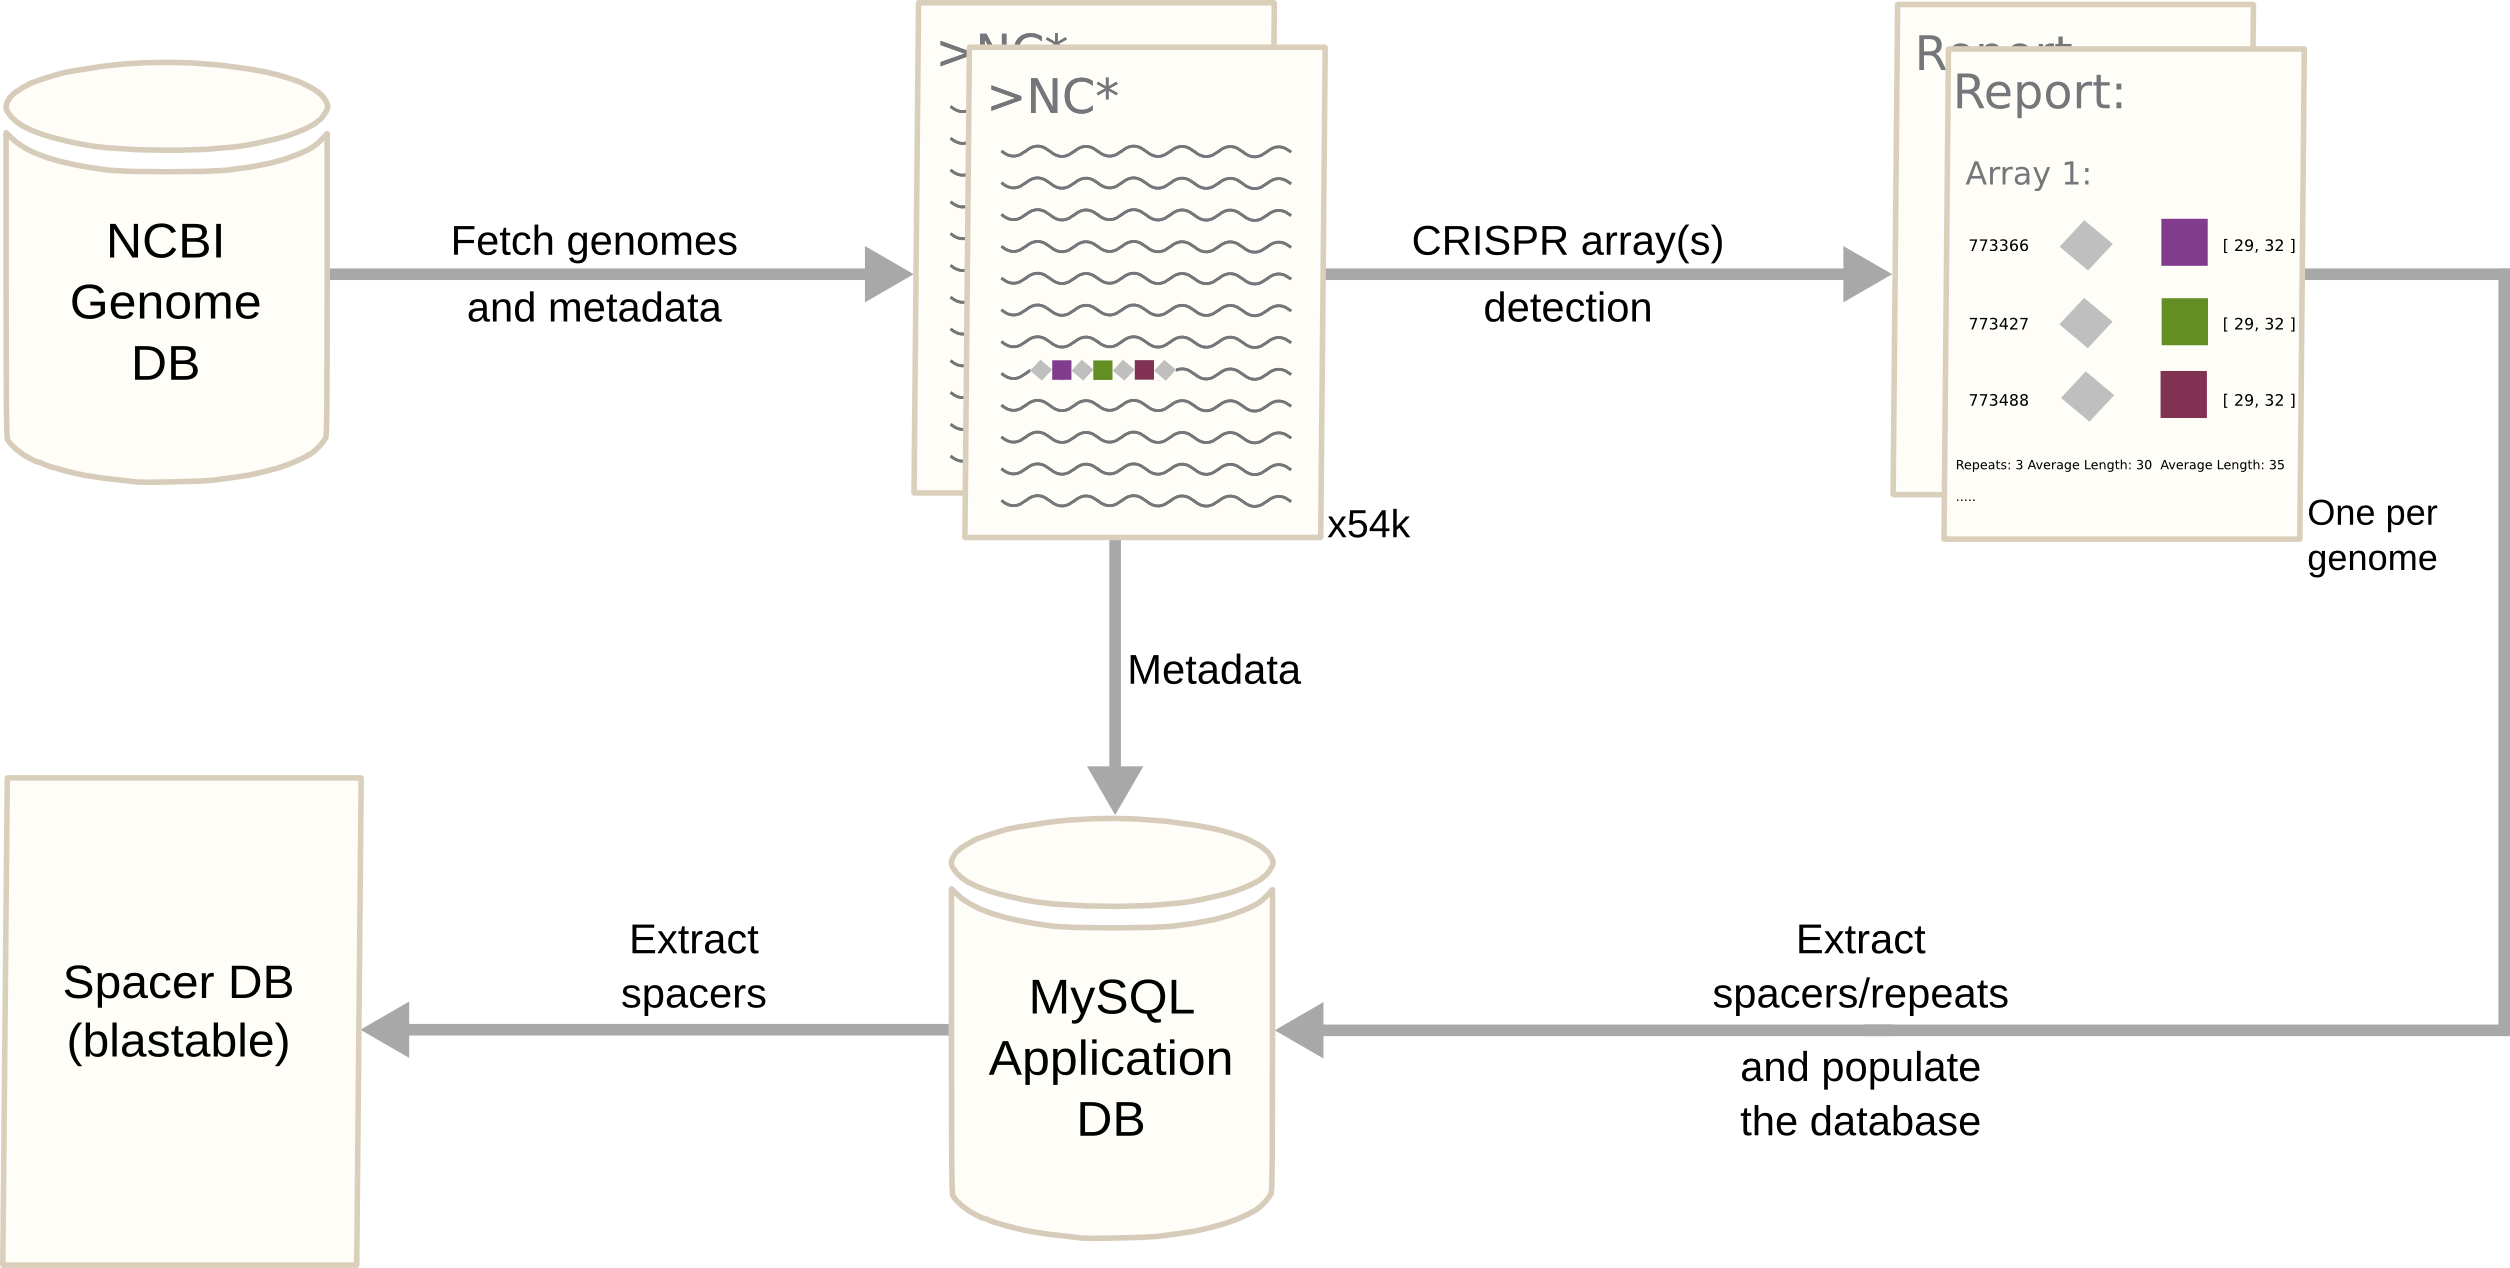
\includegraphics[scale=0.5]{figures/pipeline.png}
  \caption{Data processing pipeline}
\end{figure}

\subsection{Software Architecture}

The approach taken to expose the database and let the user interact
with the data was to develop a web application. We used Django to
accomplish that. Django is a free and open-source, Model-Template-View
(MTV) web application framework written in python, which encourages
rapid development and clean, pragmatic design. The web application is
running on a server using Apache HTTP server.

A key element of the web application is the REST API which allows the
users to programmatically query the MySQL database in order to obtain
the data for downstream analysis. This was done using the django REST
framework, a flexible toolkit for building Web APIs.

As an additional service, users have the option to blast their own
sequences against our database of spacers elements. They can also
submit their bacterial or archaeal sequences for CRISPR array(s)
detection using the CRT software installed on the server. In order to
efficiently handle user requests for BLAST and CRT services, the
requests are queued before they are run by the server's backend,
allowing for more control over the tasks and their resource usage. It
also provides the option to run them asynchronously. This element was
developed using Celery as a task queue and RabbitMQ as a message
broker.

We used free and open-source softwares to achieve our goal. We also
chose to publish our code on github, under a public license. Special
attention and care were given to reproducibility. As such, the code
was well documented. Moreover, the environment was also fully
documented using an “infrastructure as code” approach with the help of
tools like Ansible. This approach eased the developement phase, and
provides enthusiast users key elements when trying to reproduce
everything from scratch on their own infrastructure.

\begin{description}
  \item[Repository address: ] https://github.com/Milt0n/CRISPR-Exposed
  \item[Website address: ] http://www.crispex.net/
\end{description}

\begin{figure}
  \centering
  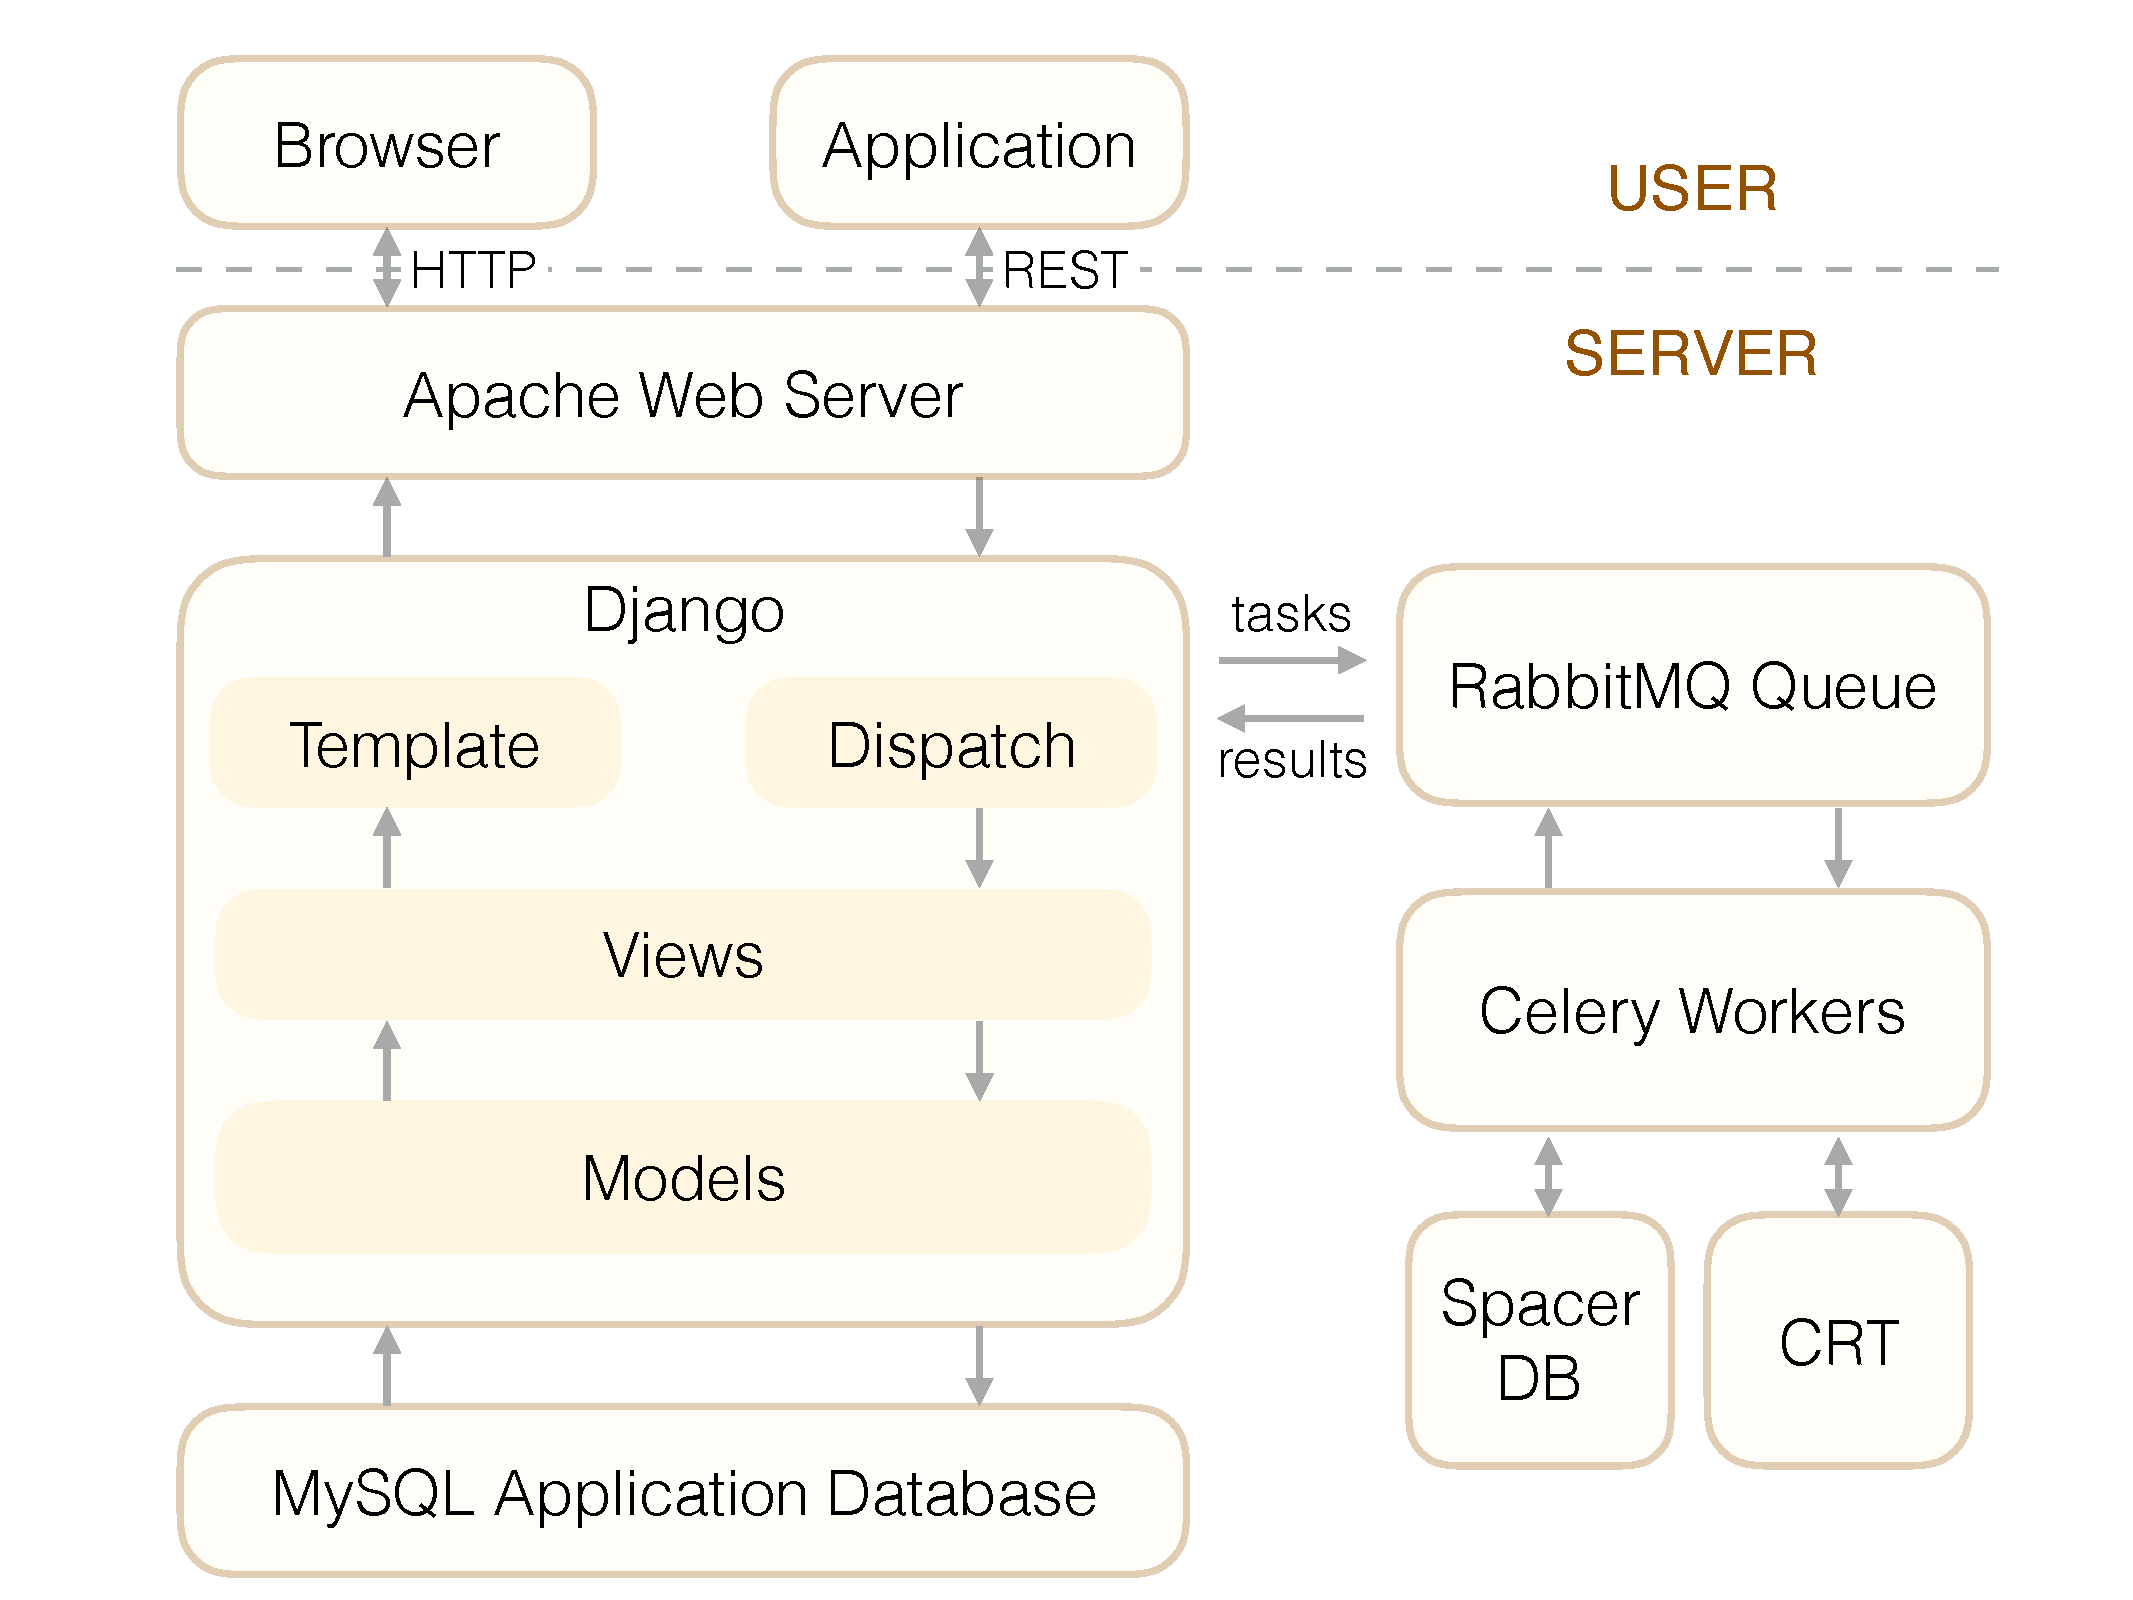
\includegraphics[scale=0.3]{figures/soft_arch.pdf}
  \caption{System Architecture}
\end{figure}

\subsection{Data Visualization}

\subsubsection{method}

Four plots were created for data visualization using D3.js
libraries. A row chart and two histograms were created using dc.js,
stable version 1.7.5 \cite{DcJs} while a parallel coordinates
visualization was plotted using parallel-coordinates version 0.7.0
\cite{ParCoordJs}. The charts were plotted using datasets in csv
format queried from the MySQL application database.

The first dataset was used to plot row chart which shows the
\emph{log10} number of genomes used in database and histograms that
shows the frequency distribution of repeats’ and spacers’ length
detected by CRT. Since these three charts were plotted using the same
data set, the information is cross-linked. Users can interactively
filter the information in these charts but it will not affect the
display in parallel coordinates.

The second data set which only consists of genomes with complete
assembly level was used to plot parallel coordinates which shows the
groups of prokaryotes, size of genomes and number of CRISPR arrays
detected per genome. Each line represent a strain, coloured by their
kingdom (i.e. bacteria in purple, archaea in orange). Axis can be
reordered and can be filtered by range.

\subsubsection{results}

The row chart shows the \emph{log10} number of genome sequences used
to populate CRISPR Exposed for each group of prokaryotes. The purpose
of showing this chart is to inform users that the content of the
database is highly biased towards some proand this should be taken
into account when interpreting the distribution of repeats’ and
spacers’ length. About half of the total of the sequences originate
from firmicutes, proteobacteria and actinobacteria. This chart could
be further improved into scale-stack row chart in the future to reduce
the cognitive load of interpreting the results.

The histograms of repeats’ and spacers’ length mainly serve the
purpose of quality control of CRISPR elements detected by CRT. Length
of direct repeats should not be deviated too much from length of
spacers. Data set used to plot the histograms was preprocessed to
remove false positive that is not bound by the constraint of parameter
settings in CRT. For instance, the maximum length of spacers for
CRISPR detection was set to 48 nucleotide long but there were about
3.6\% (28663 out of 790903) of total number of spacers detected by CRT
is longer than the length specified. These entries were stripped from
the data set to avoid misleading information.

Finally, parallel coordinates shows that most of the complete assembly
genomes available in the database have sizes around 2-7 million bp
long and contain 1 to 5 CRISPR arrays. No notable correlation between
number of CRISPR arrays and genome size was observed.

\section{Discussion}

The application and the database attached to it is novel in a couple
of ways. To our knowledge, it is the first time such an extensive
identification of CRISPR elements is conducted. About 54,000 genomes
were used in this analysis. Other projects such as CRISPRdb
\cite{grissa2007crisprdb}, and CRISPI \cite{rousseau2009crispi} only
focus on the subset of genomes that have complete level assembly
(4,000 genomes for CRISPRdb, 1,200 for CRISPI). As such, the spacer
database constructed is the largest presently available online,
consisting of 800,000 spacer sequences. We hope it can be useful to
researchers, and can envision a couple of uses of our dataset:


\begin{itemize}
\item Comparative analysis of CRISPR arrays at species, class, or
  phylum level
\item Distribution of the origin of spacers in given bacteriophages,
  or plasmids
\item Phage host prediction
\end{itemize}

\noindent Future work could include:

\begin{itemize}
\item CRISPR-Cas systems identification and classification
\item PAM sequences information
\item Detection of anti-CRISPR genes
\end{itemize}

Building upon those features, improvement in data visualization would
be welcome in order to bring further insights to users. Additional
information that could be interesting to be visualized include:
\begin{itemize}
\item Cas genes detected: it is possible that CRISPR arrays detected
  is not associated with any cas genes in near proximity. Such arrays
  may be degenerated or have other functions
  \cite{mandin2007identification}
\item Displaying the type of CRISPR-Cas systems: Each type of
  CRISPR-Cas systems have distinctive features. Displaying the type
  of CRISPR-Cas systems allows generalization of the
  whole.\cite{makarova2011evolution,makarova2015updated}
\item Information about secondary structures of repeats: Kunin et
  al. clustered putative secondary structures of crRNA based on
  sequence similarity and ability to form stable secondary structures
  \cite{kunin2007evolutionary}. Combining this information from the
  cas genes and the repeats may provide insights on function and
  regulation of CRISPR-Cas systems.
\item Protospacer-adjacent-motifs (PAM) sequences: the selection of
  protospacers from invading DNA was shown to be determined by
  recognition of PAMs which is several nucleotides long and varies
  between different CRISPR-Cas systems
  \cite{mojica2009short,deveau2008phage}
\end{itemize}


\newpage
\bibliographystyle{ieeetr} 
\bibliography{bib-db}
\end{document}
